\section{问答与工程落地}

\begin{importantbox}{本章核心判断}
AMemGym 的收束结论很直接：长程对话记忆评测的核心价值在于把 agent 放回它亲自参与的对话轨迹中，观察它怎样写入、读取、使用记忆，并把失败位置反馈给后续优化。工程落地时，短对话可以优先使用 native long-context LLM；对话变长、记忆状态频繁变化时，AWE 类方案更值得优先试验，但仍需用诊断指标持续检查 write、read、utilization 三个环节。
\end{importantbox}

\subsection{四条 takeaway：从评测到优化闭环}

结尾页把全文压缩成四条可执行判断。第一，on-policy evaluation 会暴露 off-policy benchmark 容易遮住的记忆问题；第二，当前模型即使具备较长上下文，在长交互中仍会出现明显 memory limitation；第三，external memory 有帮助，write/read/utilization 之间仍存在基础 trade-off；第四，self-evolution 具有潜力，agent 可以利用 AMemGym 的反馈迭代改善自身 memory policy。

\begin{figure}[H]
  \centering
  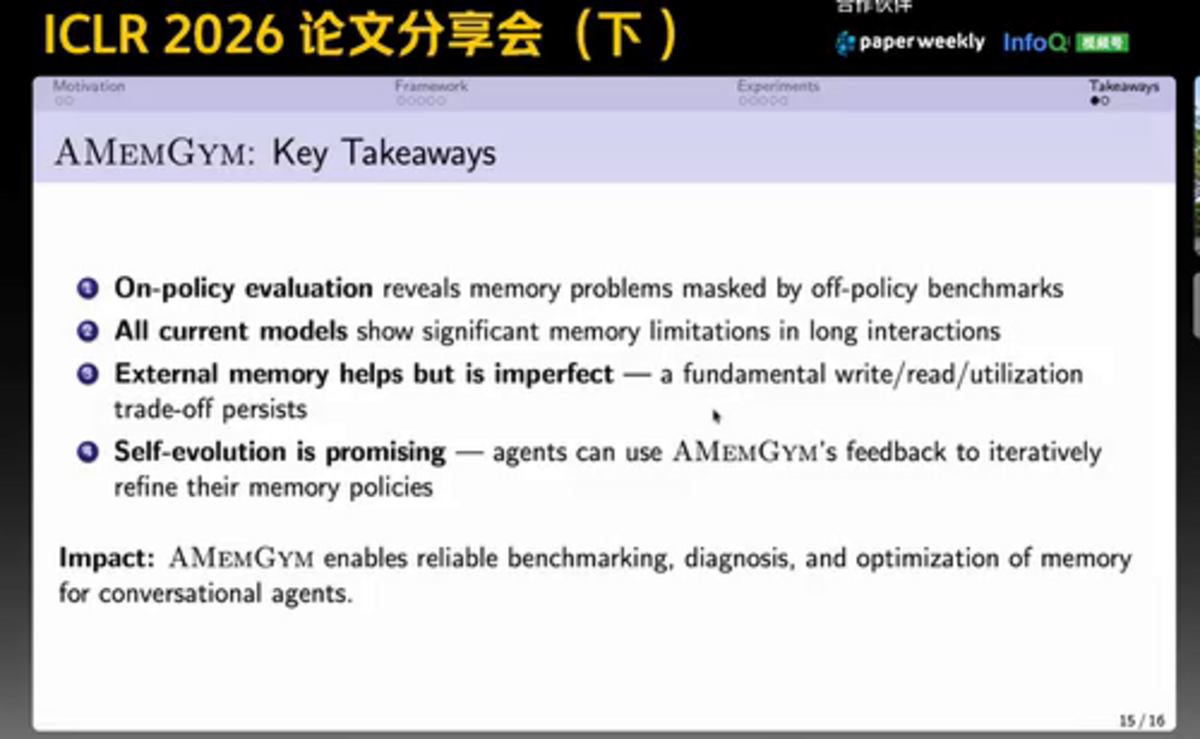
\includegraphics[width=0.82\linewidth,height=0.34\textheight,keepaspectratio]{figures/fig10_key_takeaways.png}
  \caption[AMemGym 的结尾 takeaway]{AMemGym 的结尾 takeaway：on-policy 评测、长交互记忆局限、外部记忆 trade-off 与 self-evolution。\protect\footnotemark}
  \label{fig:key-takeaways}
\end{figure}
\footnotetext{视频时间：00:19:00--00:20:42。}

图~\ref{fig:key-takeaways} 的四条并列结论背后有同一条主线：记忆系统会改变未来对话，未来对话又会改变可写入的记忆材料。评测如果只让模型阅读一段固定脚本再回答问题，就像只检查自动驾驶系统能否读懂事故报告；更关键的检查发生在系统真正控制车辆时，因为每一次转向都会改变下一秒的路况。长程对话 agent 也是这样：它上一轮是否记住用户偏好，会影响下一轮问什么、答什么、存什么。

\begin{knowledgebox}{为什么 evaluation mode 是根因}
前文已经建立 evaluation mode 的核心差异：固定轨迹答题测的是读取既定历史，亲自参与轨迹后的答题测的是闭环交互记忆。问答部分的价值在于把这一区分重新落到 benchmark 设计上：数据来源一变，optimization signal 的含义也会改变。
\end{knowledgebox}

\subsection{Q\&A：evaluation mode 是核心差异}

问答部分首先追问 AMemGym 与传统静态 benchmark 的本质区别。回答中的高信息点集中在 `evaluation mode`：传统 benchmark 往往给 agent 一段预写对话，再询问记忆问题；如果 agent 本身存在记忆缺陷，这个缺陷在真实交互中会改变对话走向，并继续改变后续可记忆内容。AMemGym 的 on-policy 设置把这种耦合关系纳入评测，因此还能输出 diagnostic feedback 与 optimization signal。

\begin{dialoguebox}{Q\&A 高信息片段（00:21:11--00:22:27）}
主持：AMemGym 相比传统静态 benchmark，在评审方式上有什么本质区别？on-policy 评测的优势体现在哪里？

Jiayang Cheng：最核心的区别在 `evaluation mode`。传统 benchmark 通常给 agent 一段预先写好的对话再提问；如果 agent 有记忆缺陷，这会影响对话走向，后续记忆内容也会被改变。on-policy 在更合理的 setting 下评估，并能提供 diagnostic feedback 或 optimization signal，用来指导记忆策略改进。
\end{dialoguebox}

这段问答值得保留，因为它把全文的抽象对比落到了评测模式本身。静态 benchmark 能检查“读过材料后能否答题”；on-policy benchmark 检查“参与互动后还能否维持正确状态”。对 long-horizon conversation 来说，后者更接近真实产品风险：客服、个人助理、协作编程 agent 的错误记忆会进入下一轮交互，随后形成连锁影响。

\begin{warningbox}{ASR 术语校正与证据边界}
本节按 outline 统一将字幕中的 “i am gm / MMGM” 写作 `AMemGym`，将 “of policy” 写作 `off-policy`，将 “native VLM / VLLM” 按问答语境写作 `native long-context LLM`。这里不补充视频未给出的模型名单、精确实验数值或论文公式；工程建议只从视频明确给出的瓶颈和问答结论向外延伸。
\end{warningbox}

\subsection{工程延伸：按对话长度、瓶颈与治理约束分流}

第二个问题追问 native long-context LLM、RAG、AWE、AWI 的核心瓶颈，以及工程落地时怎样选。视频给出的直接建议是：如果对话不太长，native long-context LLM 的长上下文能力已经带来显著提升，可以先用；对话比较长时，可考虑 AWE。这个建议需要配合三类失败指标一起读，因为一个系统整体分数高，仍可能在写入、读取或利用某一环节埋下风险。

下表的“主要瓶颈”列只保留视频机制与问答直接支持的说法；右侧列是面向产品落地的工程延伸，用来提示评估时还要检查哪些约束。

\begin{center}
\begin{tabular}{p{0.22\linewidth}p{0.34\linewidth}p{0.34\linewidth}}
\toprule
\textbf{方案} & \textbf{主要瓶颈} & \textbf{适合的工程场景} \\
\midrule
native long-context LLM & 信息都在上下文中，短对话读取压力较小；对话变长后，海量上下文中的有效利用会变难。 & 对话长度可控、记忆更新不频繁、希望先降低系统复杂度时优先试验。 \\
RAG & 原始对话直接进入检索系统，缺少写入前筛选，检索时可能带入 noisy context。 & 资料更新频率高、需要外部可维护存储、可以承担检索工程与评测成本时使用；工程延伸中还要设计摘要、元数据、删除和隐私边界。 \\
AWE & agent 自主决定哪些信息写入 external memory bank，视频中表现更均衡，也被问答部分称为长对话场景中更值得考虑的方案。 & 长对话、用户状态持续变化、需要细粒度诊断反馈来迭代 memory policy 时优先考虑；工程延伸中还要补充写入策略审计、权限和安全约束。 \\
AWI & 记忆被压缩进 in-context buffer，固定容量压缩会损失细节，读取阶段可能受影响。 & 适合轻量压缩和上下文内携带，不适合要求高保真追踪大量细节的场景。 \\
\bottomrule
\end{tabular}
\end{center}

作为工程延伸，实际选型还要看视频之外的约束。成本决定能否承受持续检索、写入策略调用和回归评测；更新频率决定 memory store 是否需要频繁增删改；隐私与安全决定原始对话能否进入外部存储；诊断反馈决定团队能否知道失败发生在 write、read 还是 utilization。如果这些约束没有被显式写进评测方案，后续优化很容易变成只调 prompt、只换模型的盲试。

\subsection{self-evolution：把诊断反馈变成优化信号}

结尾还提到一个前景方向：agent 可以利用 AMemGym 的反馈迭代优化自身记忆策略。视频只把它作为 pilot study 和未来方向提出，因此这里应保持克制：它说明 AMemGym 不只产出一个 leaderboard 分数，还可能产出可被 agent 或开发者吸收的训练信号、策略修订信号和失败定位信号。

可以把这件事想成软件测试里的失败报告。普通测试只告诉开发者“有用例失败”；更好的测试会指出失败发生在输入解析、状态更新、检索排序还是最终决策。AMemGym 的 diagnostic metrics 也是这个角色：`write failure` 指向该写没写或写错；`read failure` 指向该取没取或取错；`utilization failure` 指向信息已经在场，最终回答仍未正确使用。

\subsection{问答小结}

本章的直接 takeaway 有四个。第一，AMemGym 的核心差异是 `evaluation mode`，on-policy 让 agent 自己参与形成被评测的轨迹。第二，短对话可以先用 native long-context LLM，系统复杂度最低。第三，长对话与高频状态变化场景应重点评估 AWE，同时继续监控 write/read/utilization 三类失败。第四，RAG、AWE、AWI 的选择不能只看总体分数，还要纳入成本、更新频率、隐私、安全和诊断反馈这些落地约束。

\section{总结与延伸}

\begin{importantbox}{全文可执行结论}
全片可以压缩成一条工程链路：先用结构化状态定义要记住什么，再让 agent 在 on-policy 交互中亲自生成轨迹，随后在 checkpoint 注入 memory query，并用 diagnostic metrics 定位失败环节，最后根据失败画像选择或改造 native long-context LLM、RAG、AWE、AWI 等记忆方案。
\end{importantbox}

\subsection{把全片机制压缩成一条执行链}

AMemGym 的方法论可以落成六步：

\begin{enumerate}
  \item 定义实体、属性、关系与 state evolution，明确哪些用户事实会随时间更新、新增或失效。
  \item 通过 user simulator 生成长程互动，让 agent 的回复进入后续上下文。
  \item 在预设 checkpoint 插入 memory query，检查 agent 是否维持了正确的个性化状态。
  \item 同时观察 QA accuracy 与 diagnostic metrics，避免整体分数掩盖局部失败。
  \item 根据 write、read、utilization 的失败画像选择记忆方案，必要时组合外部存储、筛选策略与上下文压缩。
  \item 重新运行 on-policy 评测，把新的失败反馈纳入下一轮 memory policy 优化。
\end{enumerate}

这条链路的意义在于把“记忆能力”拆成可测试、可归因、可迭代的系统能力。没有 schema，测试会缺少可控事实；没有 on-policy trajectory，测试会漏掉 agent 行为对未来上下文的影响；没有 checkpoint query，记忆状态无法被精确抽查；没有 diagnostic metrics，工程团队只会看到一个模糊分数。

\begin{knowledgebox}{写、读、用的直觉类比}
`write` 像会议中做笔记：重要事实需要被正确记录；`read` 像会后找笔记：正确事实需要能被检索或带回上下文；`utilization` 像拿着笔记做决策：事实已经在眼前，回答仍要真正用上它。许多 memory agent 的失败来自第三步，因为模型表面回答流畅，内部状态已经偏离用户事实。
\end{knowledgebox}

\subsection{工程延伸：从论文结论到产品决策}

如果把 AMemGym 用在真实产品里，下面这一段属于工程延伸：最低可行流程可以从三张表开始。第一张是 memory schema 表，列出用户事实、偏好、约束、有效期与冲突解决规则。第二张是 evaluation mode 表，明确哪些用例必须 on-policy 运行，哪些短程回归可以用静态样本快速筛查。第三张是 failure ledger 表，把每次失败归到 write、read、utilization，并记录触发条件、复现轨迹和修复策略。

\begin{warningbox}{只看 overall score 的风险}
overall score 适合做入口指标，不能承担全部诊断任务。两个系统可能总分接近，一个主要漏写事实，另一个能写能读却在回答时误用事实；它们需要的修复路径完全不同。若评测报告没有 failure breakdown，工程团队会把结构性记忆问题误判成随机回答波动。
\end{warningbox}

对团队负责人来说，最终决策可以更朴素：先确认对话长度和记忆更新频率；再确认是否允许外部 memory store；然后跑一轮 on-policy 诊断；最后按失败画像选方案。短、低风险、低更新场景从 native long-context LLM 起步。长、高更新、需要长期个性化的场景，优先评估 AWE，并为 memory write 设置审计、权限、过期和删除机制。RAG 适合需要外部资料管理的系统，但必须把检索噪声、chunk 策略和隐私边界写进测试。AWI 适合作为轻量压缩策略，面对细节密集的长期记忆任务时需要谨慎。

\subsection{来源边界与使用建议}

本讲义的证据层级需要说清楚。视频直接支持的内容包括：AMemGym 的 on-policy 评测定位、三阶段框架、AWE 在 on-policy 与 off-policy 下的排序差异、后期 period 的记忆退化趋势、RAG/AWE/AWI 的外部记忆对比，以及 utilization failure 从约 24\% 降到约 7\% 这一口述结果。讲义中的产品流程、权限、过期、删除和审计建议属于工程延伸，作用是帮助读者把论文型评测转化为上线前检查清单。

读者使用这份 PDF 时，可以把它当成一张路线图：先看第 1--2 章理解为什么固定轨迹评测会低估真实交互风险，再看第 3 章掌握 AMemGym 怎样构造 ground truth 与 checkpoint query，随后用第 4--5 章的实验结果判断评测模式和外部记忆方案会怎样改变结论，最后回到本章的选型建议。这样的阅读顺序能避免一个常见误判：只盯总体分数，忽略 write、read、utilization 三个环节的失败画像。

还有一个隐含风险值得提前暴露。on-policy evaluation 更接近真实部署，同时成本、随机性和复现实验压力也更高；user simulator、状态演化规则、checkpoint 选择都会影响结论。严肃落地时，团队应把这些配置写进评测报告，至少记录对话长度、period 划分、实体 schema、查询类型、外部记忆策略和失败归因标准。缺少这些元数据时，分数很难被复查，也很难指导下一轮 memory policy 调整。

\subsection{本章小结}

最终 takeaway 是：AMemGym 把长程 agent memory 从“答对多少题”的单点评测，推进到“在闭环互动中怎样写、怎样读、怎样用”的系统诊断。可执行结论只有一句：任何准备上线长期记忆能力的 agent，都应先明确 evaluation mode，再用 checkpoint memory query 和 diagnostic metrics 找到失败环节，随后按场景约束选择 native long-context LLM、RAG、AWE 或 AWI，并把每轮诊断结果送回下一轮记忆策略优化。
